

\documentclass[a4paper,12pt]{report}
\usepackage{graphicx}
\usepackage{algorithm}
\usepackage{algorithmic}
\usepackage{fancyhdr}
\usepackage{cite}
\usepackage{epsfig}
\usepackage{subfigure}
\usepackage{setspace}

\setlength{\topmargin}{-13mm}
\setlength{\headheight}{6mm}
\setlength{\headsep}{7mm}
\setlength{\textheight}{245mm}
\setlength{\oddsidemargin}{10mm}
\setlength{\textwidth}{150mm}
\setlength{\marginparwidth}{0.5in}
\renewcommand{\baselinestretch}{1.5}
\pagestyle{fancy}
\fancyhead{}
\fancyfoot{}
\renewcommand{\headrulewidth}{0pt}
\renewcommand{\footrulewidth}{0pt}
\setlength\fboxsep{1pt}
\setlength\fboxrule{0.25pt}

\usepackage[colorlinks]{hyperref}% hyperref should be the last package to be included, and perhaps there should be one line gap between entries of bibliography
\hypersetup{
hypertexnames=false,
% pdftitle={Seminar Report},
pdfauthor={Prateek Agarwal},
%pdfkeywords={redundant, manipulator, hyper, path, planning, collision, avoidance},
% bookmarksnumbered,
pdfstartview={FitH},
colorlinks=true,
% urlcolor=cyan,
urlcolor=black,
linkcolor=black,%: Color for normal internal links
anchorcolor=black,%: Color for anchor text.
citecolor=black,%: Color for bibliographical citations in text
filecolor=black,%: Color for URLs which open local files
}%

\usepackage[nottoc]{tocbibind}

\begin{document}
\pagenumbering{roman}
\fancyfoot[CO]{\thepage}
%*******************************************************************************

\titlepage
\begin{center}

\noindent {\bf{\Large{Using DPDK to build 5G Data plane - UPF}}}\\
 {\bf{\Large{and RAN emulator}}}\\
\end{center}
\vspace{25mm}
\begin{center}
A Project Report Submitted\\
in the Partial Fulfilment of the Requirements
\\
for the Degree of
\\
\vspace{30mm}
{\bf {\large Master Of Technology}}
\\
by
\\
{\bf{\Large Prateek Agarwal}}\\
\end{center}
\vspace{20mm}
\begin{figure}[h]
\centering

\includegraphics[width=0.25\textwidth]{./fig/iitblogo.png}

\end{figure}
\begin{center}
\vspace{3mm}
{\bf {\large {Computer Science and Engineering}}}\\
\vspace{2mm}
{\bf {\large {Indian Institute of Technology Bombay}}}\\
\vspace{3mm}
{\textbf{ June, 2021}}\\
\end{center}
		% First Inner Page
\newpage
% \input{FirstFewPages/dedic}		% First Inner Page
% \newpage
\setcounter{page}{3}
%\addcontentsline{toc}{chapter}{Abstract}
% 
\textbf{
\begin{center}
\vspace{30mm}
Abstract
\end{center}
}

% This work presents a path planner for serial manipulators with large number of degrees of freedom, working in cluttered workspaces. Based on the variational principles, this approach involves formulating the path planning problem as constrained minimization of an energy based functional. The functional consists of terms representing the total joint movement and a measure of collisions over the complete path. We use semi-fixed boundary conditions at both ends of the trajectory to find more suitable start and end configurations. The concept of monotonic optimality is introduced in order to optimize the manipulator paths between the resulting end configurations. For obstacle avoidance, volume and proximity based penalizing schemes are developed. The presented planner uses a global approach to search for feasible paths and at the same time involves no pre-processing task. A variety of test cases have been presented and compared with another variational calculus based planner in order to establish the efficiency of the presented scheme in providing good quality paths.


% \newpage
%\addcontentsline{toc}{chapter}{Certificate}
% \input{FirstFewPages/MyCertificate}	
% \newpage
%\addcontentsline{toc}{chapter}{Acknowledgements}
% %\titlepage
%\begin{center}
%\mbox{}\\ 
%\vspace{3.0in}
%
%{\bf{\it{Dedicated to}}}\\
%\vskip .2in
%{\bf {\Large All my friends and well-wishers.}}
%\end{center}
%


\begin{center}
\begin{large}
{\it{\bf ACKNOWLEDGEMENTS} }
\end{large}
\end{center} 
\textit{I would like to express my sincere gratitude to my thesis guide Dr. Mythili Vutukuru for her guidance, invaluable suggestions and critical remarks for improving the quality of work. I would also like to thank my teammates Nilesh and Diptyaroop for a smoother entry to the project.}



\vskip 0.5in
\begin{flushright}
Prateek Agarwal\\
April, 2020
\end{flushright}

\tableofcontents
%\addcontentsline{toc}{chapter}{List of Figures}
\listoffigures
%\addcontentsline{toc}{chapter}{List of Tables}
% \listoftables
\newpage
\pagenumbering{arabic}
\fancyhead[RO]{\thepage}
\fancyhead[LO]{\slshape \leftmark}
\fancyfoot[CO]{}
\renewcommand{\headrulewidth}{0.5pt}
%***************************************************************************

\chapter{Introduction \label{backgr}}
5G forwarding plane and the relevant network functions are 
briefly reviewed in \ref{sec:5GfwdPlane}. PFCP protocol and its 
significance is discussed in \ref{sec:PFCP}. 
The layout of the report is outlined in \ref{sec:Organization}. 

\section {5G Forwarding Plane \label{sec:5GfwdPlane}}
The major difference in  data packet processing between 5G and earlier standards is control-user plane 
separation and the use of network function virtualization. Forwarding of packets (user plane), 
authentication of mobile devices (control plane), session establishment and management (control plane) are some of the network 
functions required in the core of a telecommunication network. These network functions run on different or same physical machines as 
virtual machines (preferably) for easier migration/scaling.

This project is mainly concerned with data forwarding plane. The network functions in our implementation will 
run as separate processes. The network functions relevant for forwarding plane are described further.
\subsection{Radio Access Network (RAN) \label{sec:RAN}} 
RAN is a point of contact for all the user equipments (UEs) like handsets, IOT devices, industrial machine controllers etc. 
RAN runs on all the mobile towers and UEs communicate with the one in their vicinity. RAN is
 responsible for talking to Access Mobility Function for authenticating the UEs, registering the  new
  session. The session establishment request is further forwarded to Session Management Function
  (SMF) which establishes a new session and forward session information to the User Plane Function (UPF). 
  \subsection{User Plane Function (UPF) \label{sec:UPF}}
  User plane function (UPF) is responsible for forwarding packets from user 
  equipments to the Internet and vice versa. Besides data forwarding, UPF also enables QoS guarantees, usage reporting, buffering etc. for data flows.
    The uplink direction is defined as the flow of the packets from user
    equipments to the Internet. The downlink direction is defined as the traffic coming from the Internet  to the user equipments/RAN. 
  
 \begin{figure}[htbp]
    \centering
    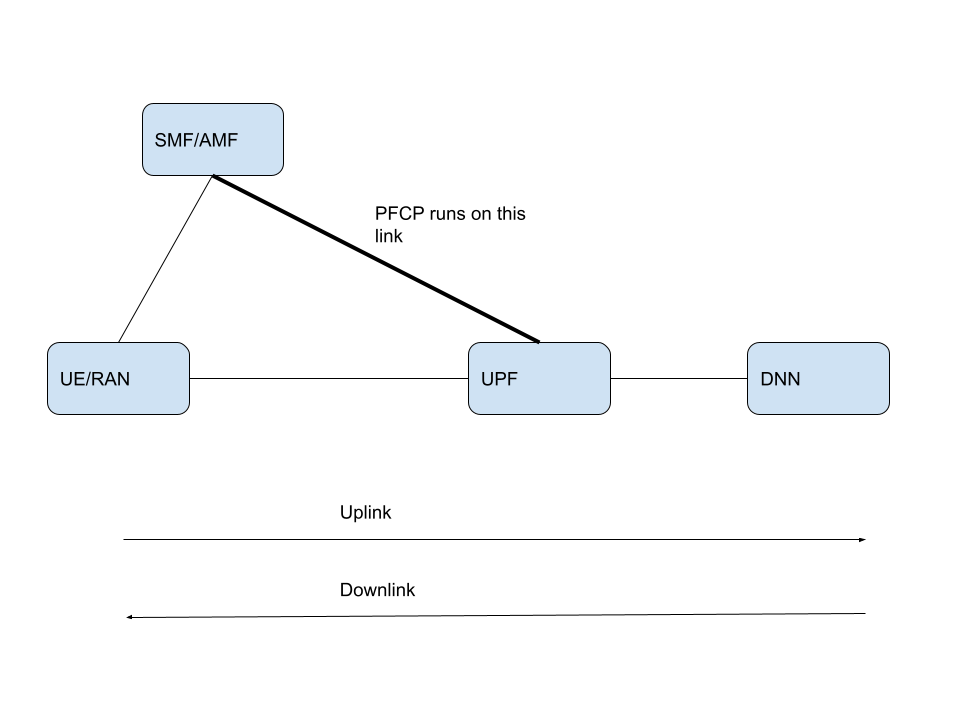
\includegraphics[width=0.7\textwidth, keepaspectratio]{./fig/Introduction/5GSecond.png}
    \caption{5G Forwarding Plane}
    \label{fig:5Gforwarding}
\end{figure}
\subsection{Data Network Name (DNN) \label{sec:DNN}}
This network function is the gateway to the public Internet. All incoming packets from outside the
 local network are received by this NF and are subsequently forwarded to the user equipment through
   the UPF and the RAN. 

\section {PFCP Protocol\label{sec:PFCP}}
 \begin{figure}[htbp]
    \centering
    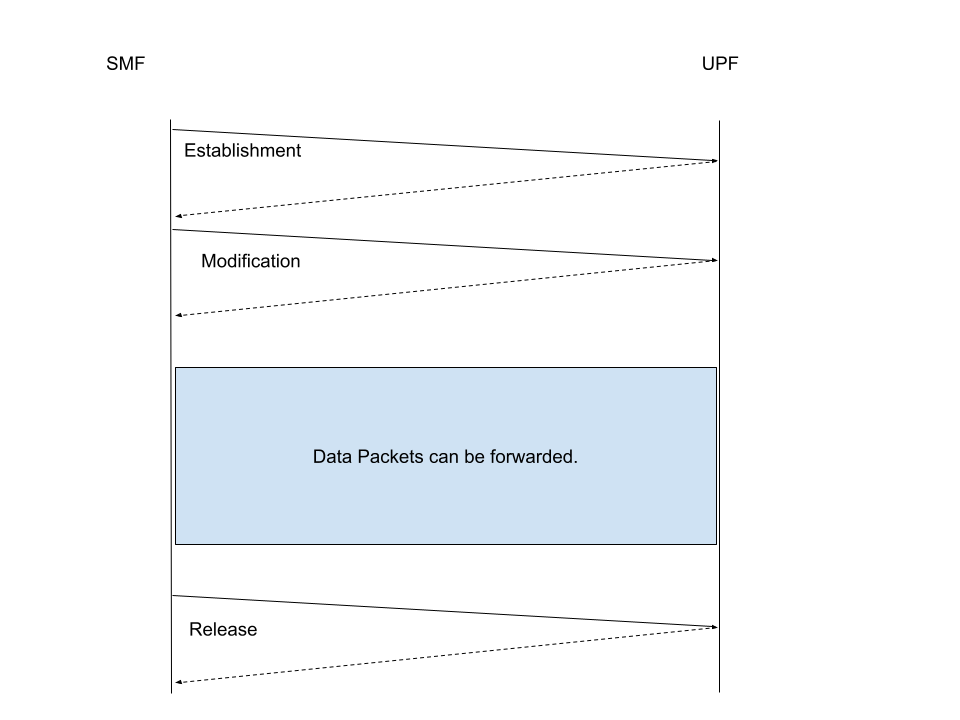
\includegraphics[width=0.7\textwidth, keepaspectratio]{./fig/Introduction/PFCP.png}
    \caption{PFCP Session Messages}
    \label{fig:PFCP}
\end{figure}

PFCP stands for Packet Forwarding Control Protocol. 
 There are two types of messages sent using PFCP - node related and session related.
 The discussion here describes session related messages.

 Session Management Function (SMF) interacts with the User Plane Function (UPF) to setup sessions related 
 information at the UPF.
This  information enables UPF to identify data packets of different sessions coming from RAN 
and provide forwarding, usage report, charging, buffering, QoS related service to the sessions.
Each session is identified by a unique session ID which helps in differentiating 
among different UEs/sessions at the UPF. 

There are three kinds of messages sent from SMF to the UPF in PFCP session related messages-
\begin{itemize}
	\item \textbf{Establishment Request} This message has all the forwarding, usage report, QoS etc. related information for  a new UE session.  
	\item \textbf{Modification Request} Once the establishment response is
	received from the UPF, the UPF sends the modification request. The important field in this message is the intimation of identifier that will be used for data plane packets coming from the UPF. The data forwarding can not start before the modification response is received.
	\item \textbf{Release Request} Once the session is not required, th release 
	request is sent to the UPF signaling the tear down of the session and UPF
	 may remove this session's related information.
\end{itemize}
UPF gives response to each of the three messages. 

\section {Organization \label{sec:Organization}}

The report is organized as follows.
The chapter \ref{chap:ProblemStatement} defines the problem statement. Chapter 
\ref{chap:RANDesign} discusses the  design of the RAN emulator describing the core
 layout, how control plane messages are forwarded and what are the different modes
  of operation. Control plane latency calculation mechanisms are explained in  the
   Chapter \ref{chap:CPLatency}. Chapter \ref{chap:CPDPTraffic} describes the
    simultaneous forwarding of control plane and data plane traffic. Chapter \ref{chap:CleanCode}  describes the steps
    taken to clean the code and make it easy to extend for future developers. 
    
     The results generated from control plane latency experiments with different models of the UPF and simultaneous transfer of control plane and data plane traffic are reported in Chapter \ref{chap:Results}.

\chapter{UPF Architecture\label{chapterUpfArchitecture}}
\begin{itemize}
	\item Feature Implementation
	\begin{itemize}
		\item Control Plane Latency Calculation.
		\item Simultaneous forwarding of Data Plane and Control Plane Traffic.
	\end{itemize}
	\item Refactor, clean and make the RAN code easy to understand and further extend.
\end{itemize}
%
%\begin{figure}[htbp]
%    \centering
%    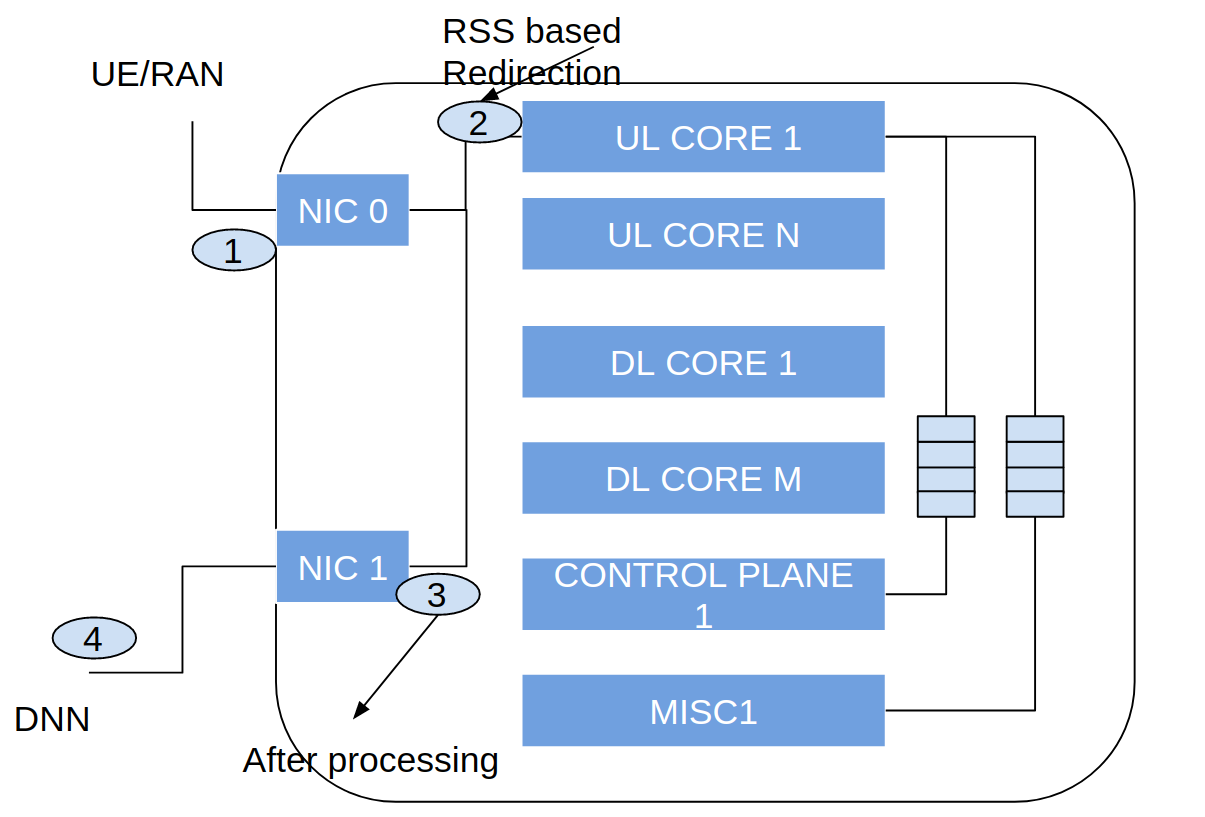
\includegraphics[width=0.9\textwidth, keepaspectratio]{./fig/Introduction/UPF2.png}
%    \caption{UPF Architecture}
%    \label{figUPF}
%\end{figure}


\chapter{Receive Side Scaling\label{chapterRSS}}

\section{What is Receive Side Scaling or RSS? \label{sectionRSSIntroduction}}
The multiple cores present on the current hardware can be used to scale the processing capability of a single node.
A packet arriving on the NIC is redirected to different cores for independent processing. This redirection may occur either
in software or hardware.
\begin{itemize}
        \item \textbf{Software} A master core receives all the packets and redirects it to multiple  worker cores. This redirection can happen in round robin or hash computation with header fields as key for the hash function (see Figure \ref{figPipeline}). 
The hash computation technique is preferred as packets of the same flow go to the same core giving better memory locality. This model is referred to as the  pipeline model of execution. 
       \item  \textbf{Hardware (on the NIC)} The hash computation on header fields happen on the NIC itself (see Figure \ref{figRTC}). This is known as Receive Side Scaling (RSS). The rest of the packet processing happens in software. The RSS computation in the context of 5G UPF uplink packet handling will be discussed.  
\end{itemize}
These alternative models of execution are discussed in Chapter \ref{chapterModelsofExecution}. 

\section{Standard RSS \label{sectionstandardRSS}}



The RSS hash for an incoming packet is computed on the transport and network layer headers. In the case of IPv4-UDP packet, the input to the hash function are IP and UDP headers. The main fields in the headers for hash computation for a GTP encpasulated packet are
\begin{figure}[htbp]
    \centering
    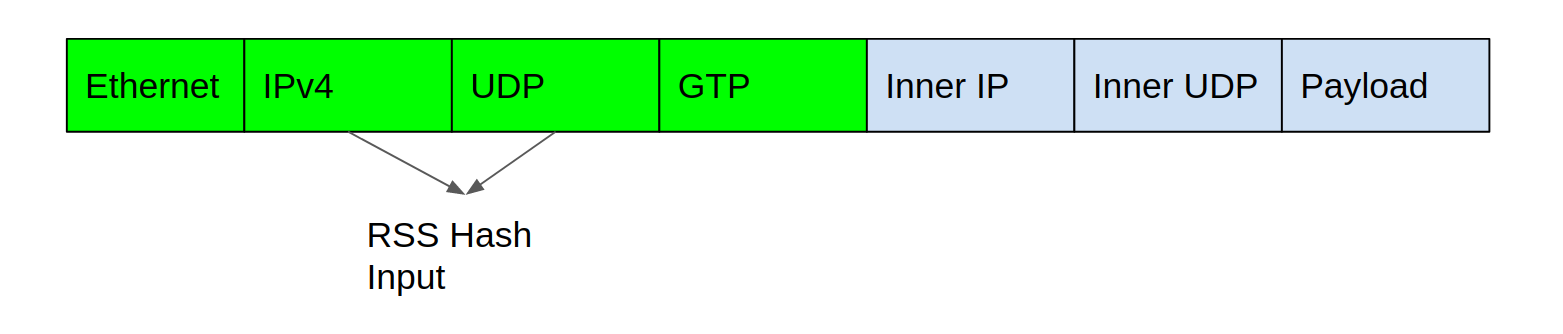
\includegraphics[width=0.7\textwidth, keepaspectratio]{./fig/Ch3DDP/noDDPpacketHashFields.png}
    \caption{Standard RSS input Fields}
    \label{figStandardRSSfields}
\end{figure}

\begin{itemize}
\item \textbf{Outer Source IP} is the RAN IP - same for all the uplink packets.
\item \textbf{Outer Source Port} In the earlier setup, this port was randomized to  get unique hash key for RSS computation. This is not a good idea as source ports are not in the control of the UPF. 
\item \textbf{Outer Destination IP} IP of the UPF - same for all the uplink packets.
\item \textbf{Outer Destination Port} is 2152 - same for all the uplink packets.
\end{itemize}
So the RSS hash key computation based on these headers will not work in our context.

\section{Alternatives \label{sectionAlternativesDDP}}
The following alternatives were explored:
\begin{itemize}
\item \textbf{Flow Director}
The 40Gbps Intel X710 NIC provides an option of inserting flow rules in the hardware itself (see \cite{flowReport}). These flow rules can be used to match different fields (including the inner payload) of the packet to make forwarding decisions. It is a better alternative than processing headers in software. However, there are two major limitations found with this approach.
\begin{itemize}
\item \textbf{Limited number of entries} Only 8k entries can be made in the flow table. The 5G use case requires us to handle UE sessions which are much larger in number. The experiments are performed for a maximum of 65536 live UE sessions. 
\item \textbf{No wildcards} Wildcard matching is not supported by the NIC. The number of flow rules could have been reduced drastically with mapping a range of UEs to a fixed core.
\end{itemize}
Due to the above limitations, the idea of using flow director was dropped. The 40Gbps NICs may support these features in future.
\item \textbf{Dynamic Device Personalization for RSS} This feature provides  the capability to parse fields of inner packet in a GTP-U packet for hash computation. This feature was exploited to get hardware based redirection and is explained in further sections.
\end{itemize}

\section{Dynamic Device Personalization \label{sectionDDP}}
Intel 40 Gbps NIC (XL710) provides the capablility to customize RSS hash key input fields \cite{ddpGuide}. RSS hash is still computed in hardware. However the fields parsed for RSS hash computation includes 
\begin{figure}[htbp]
    \centering
    \includegraphics[width=0.7\textwidth, keepaspectratio]{./fig/Ch3DDP/DDPpacketHashFields.png}
    \caption{DDP RSS input Fields}
    \label{figDDPRSSfields}
\end{figure}


\begin{itemize} 
\item \textbf{Inner Packet IP fields} Every UE has different source IP. It may not be unique for multiple sessions by the same UE. Still it has good randomness.
\item \textbf{Tunnel ID in GTP header} This field is unique for every session. 
\end{itemize}
So a combination of the above two tuples generates enough randomness for redirection of packets on different cores. 
As the name suggests, this feature/profile can be dynamically loaded and removed from the NIC during the execution of the program. There are no permanent changes made to the NIC configuration.
Note that this feature can also be used with Flow Director (discussed in section \ref{sectionAlternativesDDP}) which was not used because of the reasons mentioned.

\section{Limitations of Dynamic Device Personalization \label{sectionlimitationsDDP}}
This feature requires exact matching of all the headers for hash computation. If a field does not follow the protocol format, the packets are directed to the first queue configured on the NIC.

\begin{figure}[htbp]
    \centering
    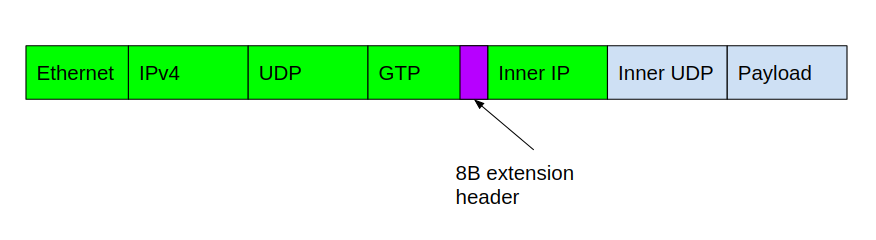
\includegraphics[width=0.7\textwidth, keepaspectratio]{./fig/Ch3DDP/ExtensionHeaders.png}
    \caption{Extension Header Limitation}
    \label{figextensionheaderLimitation}
\end{figure}

The extension header is used in our case for  providing QoS aggregate maximum bit rate (AMBR) that is allowed per session. The parsing of the GTP packet fails due to the presence of the extension header and all packets are directed to the first queue.
This is the limitation of the hardware and may be addressed in future by programmable switches or customized DDP feature prvided by hardware vendor (Intel in this case).
The experiments performed during this project are not providing different AMBRs for different sessions. AMBR is set above the incoming rate. As a workaround, no extension header is used and AMBR is implicitly assumed. The pipeline model does not have this limitation and the extension headers are used.













%    \centering
%    \includegraphics[width=0.7\textwidth, keepaspectratio]{./fig/c3f1.png}
%    \caption{DPDK: Packet movement}
%    \label{fig1c3}
%    \end{figure}
%\section{Introduction} 
%Poll Mode Drivers (PMD) are the user space network drivers. The device drivers are a piece of software which knows how to 
%interact with an external device like hard disk, CD-ROM, and NIC among others. The network drivers are the device drivers which interact with network devices like NICs. DPDK has drivers compatible with 1 Gigabit, 10 Gigabit and 40 Gigabit Intel NICS. DPDK also has drivers compatible with \emph{virtio} - a virtual device used for interacting with virtual machines.
%
%
%\section{Background: Interaction between a Driver and a Device \label{backdriver3}}
%The device and the driver store data and control information like statistics, debugging or error status at two places-
%\begin{itemize}
%    \item Base Address Registers (BARs) on the device (NICs in our case). These are primarily used to store control information.
%    \item Main Memory Locations. The data (packets) are primarily stored here. 
%    \end{itemize}
%The data is transferred with the help of
%\begin{itemize}
%        \item \textbf{Memory-Mapped IO (MMIO)} The BARs or RAM location used for data transfer are placed in the shared address space. The user process or driver can communicate with BARs or shared memory by reading or writing on these addresses. Similarly the device (NICs) can write (read) data packets to (from) these shared memory regions using DMA transfer. 
%        \item  \textbf{x86 IO ports} Data can also be transferred by writing to registers using \emph{x86 in and out instructions}. This technique is not used with modern NICs. However it is used along with MMIO in virtio implementation by writing memory addresses in IO registers in igb\_uio drivers (section \ref{uio3}).
%    \end{itemize}
%    \subsection{Transfer of Packets}
%    \subsubsection{Hardware NICs \label{nic3}}
%NICs have multiple receive and transmit queues. Incoming traffic is distributed among different receive queues by using hashing technique. Multiple transmit queues generally combine into one queue per interface before transmitting packets.
%A simple model of one receive queue and one transmit queue is assumed in the following description.   
%\begin{figure}[htbp]
%    \centering
%    \includegraphics[width=0.7\textwidth, keepaspectratio]{./fig/c3f2.png}
%    \caption{DMA descriptors \cite{ixydpdk}}
%    \label{fig2c3}
%    \end{figure}
%The driver allocates space for a circular array for holding pointers to the physical address of the data packets. These pointers are called \emph{DMA} descriptors (see Figure \ref{fig2c3}). Packets are moved by passing these descriptors between NIC and driver with the help of a head (owned by NIC) and a tail (owned by driver) pointer. 
%A buffer table (Figure \ref{fig3c3}) which maps physical addresses to virtual addresses is also maintained. This mapping is required on packet reception as the user process uses virtual addresses. The packets are processed in batches.
%\begin{figure}[htbp]
%    \centering
%    \includegraphics[width=0.7\textwidth, keepaspectratio]{./fig/c3f3.png}
%    \caption{Layout of a receive queue \cite{ixydpdk}}
%    \label{fig3c3} 
%    \end{figure}
%
%
%Transmit side is similar except for the asynchronous transfer of packets on to the links. The process returns after filling the packets on the ring. When the packets are transmitted later, the driver is notified by the movement of pointers on the circular buffer. The sent packets are subsequently freed or erased and returned back to memory pools (\ref{mempool4}). 
%\subsubsection{\emph{virtio} queues}
%\emph{virtio} queues are used to transmit data packets between host machine and virtual machines.  Packets are received/transmitted by storing them in DMA buffers (section \ref{nic3}). However virtio queues (that store DMA descriptors) consists of two rings- \emph{available} and \emph{used} (see Figure \ref{fig4c3}).
%% On the transmit side, the packets' descriptors are inserted in the 
%The \textbf{available} ring is used for receipt/transfer of packets. Once the packets are processed, the descriptors are kept in the  \textbf{used} ring . The network driver then clears the descriptors and which can then be reused.
%The \textbf{available} queue indices are written in device registers using \emph{IN/OUT} x86 instructions. 
%\begin{figure}[htbp]
%    \centering
%    \includegraphics[width=0.7\textwidth, keepaspectratio]{./fig/c3f4.png}
%    \caption{Virtio Queues \cite{ixydpdk}}
%    \label{fig4c3} 
%    \end{figure}
%The virtio queues are not exclusively used for packet transfers. For example, virtio queues are also used for reading files from disk. The transmit function prepends a header to the network data. This header helps the driver in differentiating network packets from other devices' data.     
%
%\section{Design of important PMDs}
%\subsection{igb\_uio \label{uio3}}
%DPDK uses \emph{uio} kernel subsystem to build \emph{igb\_uio}\cite{memblogdpdk2} driver. This driver is used for both virtio and hardware NICs \cite{ixydpdk}. \emph{uio} provides full access to the shared registers and shared memory by memory mapping these regions into files. These files are located in \emph{sysfs} virtual-filesystem (VFS). \emph{sysfs} treats an external device as a file.
%\subsection{vfio-pci-driver}
%DPDK uses \emph{vfio} kernel subsystem to build \emph{vfio-pci} driver. vfio provides IOMMU support for virtualized environments. IOMMU is a memory translation unit present on NICs  which directly maps guest virtual addresses to host physical addresses. This enables NICs to perform DMA directly and guest VMs can interact with devices using guest virtual addresses. 
%\subsection{Software PMDs \label{softpmd3}} 
%DPDK also has PMDs which do not require kernel subsystems like uio or vfio. These PMDs are built over packet capture libraries
%like \emph{libpcap} and \emph{AF\_PACKET} \cite{afpacket} sockets. The packet capture framework allows DPDK to work with any hardware by providing raw packets to the driver. 
%
%
%
%
%
%\section{Configuration and Device Statistics}
%DPDK PMDs provide APIs for configuring and collecting device statistics from NICs (Figure \ref{fig5c3}).
%\begin{figure}[htbp]
%    \centering
%    \includegraphics[width=0.7\textwidth, keepaspectratio]{./fig/c3f5.png}
%    \caption{Control APIs}
%    \label{fig5c3} 
%    \end{figure}
%\subsection{Configuration \label{config3}}
%Depending on the capability of hardware NICs, the NICs can be configured for
%\begin{itemize}
%    \item \textbf{Offloading Calculations} - Checksums, CRC checks, VLAN tag processing among others.
%    \item \textbf{Directing Traffic} - Destination lookup and making forwarding decisions like dropping packets, diverting it to a specific queue,  packet encapsulations for tunnel offloads (IPv6 packet inside a IPv4 packet for transmitting on an IPv4 compatible link) and so on.
%\end{itemize}
%This is performed with the help of APIs which are present in Flow Library\cite{progguide}. 
%
%\subsection{Device Statistics}
%PMDs provide APIs for collecting statistics on the network traffic. The statistics include but are not limited to number of incoming packets, number of transmitted packets, packet drop rate etc. The extended statistics API is used for getting statistics which are unique to a device.
%
%It is the responsibility of application developer to use these statistics or configure the hardware if required. The PMDs act as the translators between application and the hardware.
%




\chapter{Models of Execution \label{chapterModelsofExecution}}
\section{Latency Calculation Algorithms}
\subsection{Key Concept}
When packets are transmitted from RAN, the timestamp when the packet is forwarded is stored for the outgoing packet. When the response for the packet arrives at the receiving side of RAN, the difference in time values of the current time and the stored timestamp  is calculated and then reported in the log file.
\subsubsection{Storing of Timestamp}
\begin{itemize}
	\item \textbf{Data Plane} The packet identification field in the IP header is used to identify the packet. These latency packets
	      are sent from the core CORE\_RTT. All the established sessions/UEs are used for forwarding the traffic. When the packet is
	      transmitted, a callback  function stores the outgoing packet timestamp in a hashmap with packet id as the key. This field is
	      generally used in the fragmentation and reassembly of packet data. The data plane latency packet throughput is substantially reduced by introducing sleep commands. The option of disabling the calculation of latency is removed as latency packets do not significantly affect any other metrics. Data plane latency is independently logged in a different column in the log file.
	\item \textbf{Control Plane}
	      This requires deep packet inspection of control plane packets. These packets are sent from the core CORE\_CP\_TRAFFIC.
	      There are three types of control plane packets - session establishment, session modification and session release packets - all of
	      them are used for measuring control plane latency. These packets have session ids stored at
	      different offsets in the payload.

	      Earlier, a hash map was used for storing the timestamps. The use of hashmap slows down the call backs and unnecessary limits the rate of data forwarding.

	      Subsequently, fixed length array was used to store timestamps - \textbf{TSArray} . The
	      array size is $65536 * 3$ and stores the value of timestamp register \textbf{rdtsc} of the
	      outgoing packets. The first $65536$ values are used to store establishment packet related
	      timestamps, next $65536$ modification packet related timestamps and then release packet
	      timestamps are stored.
	      The bitwise operations can be easily used as 65536 is a power of 2.


	      A callback function is registered on  the transmit queue corresponding to CORE\_CP\_TRAFFIC which stores the timestamp in the hashmap.
\end{itemize}
\subsection{Calculation of Latency}
A single callback function is registered on the CORE\_RX\_POLL which  receives the incoming packet.
\begin{itemize}
	\item \textbf{Data Plane} The same outgoing packet is reflected by the DNN packet and stored timestamp is retrieved from the hashmap and the difference is the end to end latency of each packet.
	\item \textbf{Control Plane} Every control plane packet has a response packet - establishment response (51), modification response (53), release response (55). The control plane latency is the time period from when the request packet is sent and the response packet is received.
	      The response packets have message type and either session IDs in their payload. For
	      modification and deletion  responses, the session ids have a difference of 3000.  Using these information, the index in \textbf{TSArray} can be calculated and the corresponding timestamp can be retrieved.
\end{itemize}
\subsection{Why do we need different techniques for control plane and data plane?}
\begin{itemize}
	\item \textbf{Why can't we use packet identifier for control plane packets?}
	      Both types of packets are received on the same rx queue/core. So, only the packet identifier in ip header is not enough to differentiate control plane and data plane packets. And you will need deep packet inspection to differentiate among the two packets.
	\item \textbf{Why don't we inspect packet payload for data plane packets?} Data plane packet has no useful payload and when the ip header identification field is unused till now, we can use it.
	\item \textbf{Development Sequence}
	      Data plane latency was implemented earlier when the packet id field was unused. Control plane latency calculation is done later.
\end{itemize}

\section{Callback functions}
Call back functions are registered on receive and transmit queues for latency calculation.
\begin{itemize}
	\item \textbf{CPStoreTimestampCallback}
	      Registered on CORE\_CP\_TRAFFIC for storing the timestamp of outgoing control plane packets.
	\item \textbf{DPStoreTimestampCallback}
	      Registered on CORE\_RTT for storing the timestamp of outgoing  data plane latency packets.

	\item \textbf{CPLatencyCallback}
	      Registered on CORE\_RX\_POLL for inspecting responses to control plane
	      requests. The difference in the current time and the  timestamp stored during the
	      tx callbacks gives the latency values.
	\item \textbf{DPLatencyCallback}
	      Also registered on CORE\_RX\_POLL for inspecting the mirrored data plane
	      latency packets.
\end{itemize}
%Run-to-Completion and Pipeline are two models of execution for packet processing and forwarding at User Plane Function.
%Comparison of these models in the different use cases/scenarios is one of the major objectives of our work. This chapter will explain these models of execution.
%
%\section{Run-to-Completion (RTC) \label{secRTC} }
% \begin{figure}[htbp]
%    \centering
%    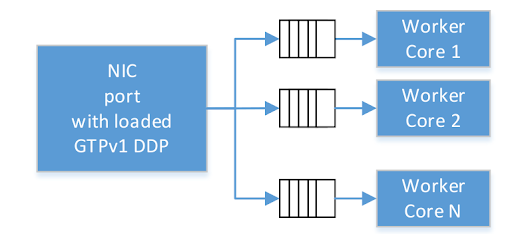
\includegraphics[width=0.7\textwidth, keepaspectratio]{./fig/ModelsofExecution/RTC.png}
%    \caption{Run-to-Completion}
%    \label{figRTC}
%    \end{figure}
%Keeping processors independent with minimal or no communication between them is the key idea of this model. Each
% processor should be able to completely recieve, process and forward/transmit the packet if required. Redirection of packets on different core requires receive side scaling (RSS) discussed in chapter \ref{chapterRSS}. Packets of a session are redirected to the same core as RSS value for packets of the same session is same.
%\section{Pipeline \label{secPipeline}}
%\begin{figure}[htbp]
%    \centering
%    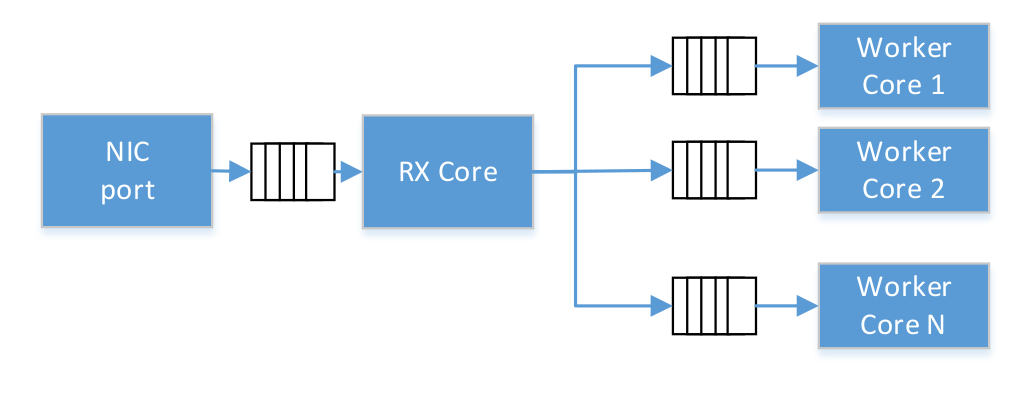
\includegraphics[width=0.7\textwidth, keepaspectratio]{./fig/ModelsofExecution/Pipeline.png}
%    \caption{Pipeline}
%    \label{figPipeline}
%\end{figure}
% Hardware based redirection is either not possible or not used in this model. Complete packet processing including redirection occurs in software. Packets are redirected to a master core which processes the outer headers to redirect packet on one of the worker cores. Generally packets of a session are redirected to the same core to maintain better spatial and temporal locality. However packets may be redistributed if a particular core gets overloaded.
%It requires inter-core communication. This communication happens through a software ring/circular queue for each worker core. The master core keeps incoming packets on the corresponding software ring of the worker core. The processed packets are then received by master core (through another ring) to transmit them over the wire.
%The pipeline model can also redistribute load by shifting load from high load core to least loaded loead.
%Our pipeline implementation handles this by mapping UEs from heavy loaded core to lightly loaded core. The UEs are remapped as long as there is no uniform distribution of load among different cores.
%\section{Comparison \label{RTCpipelineComparison}}
%
%The RTC has some significant advantages over the pipeline model.
%\begin{itemize}
%    \item \textbf{Better Throughput} The per core processing capability is expected to be higher in RTC model. This is due to no inter core communication and
% hardware support for hash computation. The computation in the hardware is generally faster than in software. This also keeps
%  CPUs meant for hash computation free for other tasks. 
%  \item \textbf{Lower Latency}The end to end latency in pipeline also takes a hit due to intercore
%   communication between master and worker core.
%\item \textbf{Easy to implement and understand} The RTC implementation's source code is easy to understand as it is same on all the cores. Pipeline has different logic and complex interaction between master and worker cores.
%\end{itemize}
% 
%However, pipeline is better suited to change operational behavior dynamically. This hypothesis is tested for two use cases.
%\begin{itemize}
%    \item \textbf{Dynamic Scaling} The key idea here is to start user plane function with minimum number of cores and vary
%     the number of cores according to the current traffic load. This helps in better energy efficiency as the cores may
%      remain idle when there is less traffic. It  is easy to reconfigure the number of cores in pipeline than RTC. RTC
%       requires stopping of ports before reconfiguring them as the number of RSS queues needs to be updated in hardware. A large number of packets are dropped during this reconfiguration. Pipeline requires the launch of cores in software which is relatively light weight.
%    \item \textbf{Redistribution of traffic}  Once flows are mapped to cores by hash output in RTC, it is not possible to redirect them to another core. This may be required when the load is
%     highly skewed towards some cores and the rest of the cores are idle. In such cases, a large number of packets are
%      dropped by heavily loaded core in RTC model. 
%    Pipeline can effectively handle such scenarios by redirecting certain flows from heavily loaded cores to less loaded cores. This reduces the number of packets dropped and better core utilisation. 
%\end{itemize}
%
%Experiments (discussed in chapter \ref{chapterExperimentsandResults}) were performed to test and evaluate these claims in 5G use case context. 
%
\chapter{Experiments and Results\label{chapterExperimentsandResults}}
This portion of the problem statement took the maximum effort and time.
The inherited code was never cleaned and had various issues which are discussed below.
\section{Naming of Variables}
\subsection{Issues}
\begin{itemize}
	\item \textbf{Wrong Case} camelCase should be used in all the 5GCore network functions. PascalCase is OK too. 
	However snake\_case, snake\_camelCase were also rampantly used in the RAN code. 
	\item \textbf{Redundancy} Having test or dpdk in the name of every function is not helpful when it is already
	a testing/experimental setup and DPDK APIs are used. 
\end{itemize}
\subsection{Resolution}
All new functions that were defined do not have these issues. The name of many past functions are also changed.
The complete revamp is avoided as past functions might be familiar to the team by the old names.

\section{Stale Comments}
\subsection{Issues}
\begin{itemize}
	\item \textbf{TODOs} There were many todos lying around from very long. 
	The one who would have these TODOs on their list might have completed them on their branch 
	or have never bothered after writing the TODOs.
	\item \textbf{Misleading Comments} The comments were not updated with the change/removal of the lines of 
	the code.
\end{itemize}

\subsection{Resolution}
Whatever TODOs and misleading comments that came in my way have been erased.
\section{Dead Code}
\subsection{Issue}
\begin{itemize}
	\item There were many functions in the code which were never called in any of the data forwarding mode.
	      Some of them were aptly identified as beta functions and many were not.
	\item Hundreds of lines of code was defined in the  conditional statement $if(0)$- they were never called/compiled.
\end{itemize}
\subsection{Resolution}
Dead code mentioned in the issue sections is cleaned.

\section{Deprecated Options}
\subsection{Issue}
There were 20 modes of data forwarding available. Hardly 3-4 were used for testing purposes. Many options 
were redundant as same options were implemented using dpdk APIs and kernel based functionalities.
\subsection{Resolution}
The number of modes are reduced to 5. They are appropriately categorized as main data forwarding modes, helper 
functions and QoS related modes. The code that is not based on DPDK APIs is removed for clarity.
\section{Copied Code}
\subsection{Issues}
DPDK provides a lot of examples showing the usage of their API. It is quite extensive and easy to read and excerpts of 
code can directly be used in our applications. The code should be cleaned when it is lifted from these applications.
The declaration of functions which are never used should be removed. The variables should be named according to
the convention that is followed in our source. The header dpdk\_ran.h had around 600-800 lines of declared functions
which were never defined and used.
\subsection{Resolution}
Most of the declarations discussed here are removed. There might be some declarations in other header files which were not removed. 
Future developers may clean whenever they come across them.
\section{Global Variables}
\subsection{Issue}
Around 150 variables, data structures were declared globally in ranMain.cpp. The use of
global variables made the code highly coupled and made it difficult to change one procedure
without affecting the other. Infact some of them were declared but never used.
This made it also difficult to discern the scope of variable usage inside a procedure - whether is s global variable,
local variable or a class member.
\subsection{Resolution}
\begin{itemize}
	\item The unused global variables are deleted. The variables which were called in only a few functions are made
	      local and passed as parameter.
	\item The remaining global variables are defined in a new namespace \textbf{Global}. This helps in identifying
	      global variables in the procedures' definitions.
\end{itemize}
\section{Directory Structure}
\subsection{Issues}
\begin{itemize}
	\item The earlier RAN directory was not created as a different folder in 5GCore folder as other NFs. 
It was defined inside AMF.  This was very misleading and suggested coupling between AMF and RAN when 
there never was. It was primarily done to avoid creating a new CMakeLists and reuse the build functionality
of AMF.
\item All log files were generated in the parent folder itself. This makes it difficult to read, delete
, transfer log files. 
\end{itemize}

\subsection{Resolution}
\begin{itemize}
	\item A different folder DPDK\_RAN is created inside 5GCore directory.
	\item Log files are now generated in subdirectories. Two log files are generated in each run - throughput 
	log files and debugging information related log files.
\end{itemize}
\section{Poor Refactoring}

\subsection{Issues}
\begin{itemize}
	\item The main function had a switch statement for different modes of operation. This switch statement was approximately 2000 lines long.
	\item The DRY principle was violated multiple times. If all modes require setting of time duration of the run, it is better to
	define a procedure asking for time rather than repeating it 20 times.
	\item The files were unusually long. The ranMain.cpp and dpdk\_ran.cpp were more than 10k,  8k lines of code respectively.
	The file in which main routine is defined should be small enough for readers of the code to grasp.
\end{itemize}	
\subsection{Resolution}
The code was extensively refactored. Differnt procedures were defined for each of the switch statement option.
Different modes were refactored to make them shorter and easy to understand. 
ranMain.cpp is bifuracted into ranMain.cpp and ran.cpp (for lack of a better name). The header ranMain.h is defined for
inclusion into both the translation units.
Further refactoring can be done of the data forwarding procedures if required. It will be a good exercise in 
understanding of the code.

\section{Unnecessary Offloads}
\subsection{Issues}
As some sections of the code were directly copied from dpdk applications, there were 
some offloads which are unrelated to our application - VLAN, QINQ and MACSEC offloads.
The entire code in dpdk\_ran.cpp was infested with these offloads. These offloads were present with IP
and UDP checksum related offloads which were used by our application.
\subsection{Resolution}
These lines of code were removed from the dpdk\_ran.cpp . However if the surgeon is not an expert,
one may remove healthy and important part with tumors as well. Thankfully, it was possible here 
to reinstall the healthy part back. This took enormous amounts of time and it was a good learning experience
for future.

\section{Technical Improvements}
\subsection{Issues}
\begin{itemize}
	\item High throughput of data plane latency packets. 100 Mbps of data plane latency packets were sent for measuring the 
	end to end latency besides the load. Law of large number comes into play much before that and high latency packet throughput 
	causes unnecessary callback overhead.
	\item The statements like \textbf{if (argc == 0)}, for loop running once, calling an internal function of the
	dpdk API when external call. 
\end{itemize}

\subsection{Resolution}
The mentioned throughput was reduced to 0.4 Mbps. This can be further reduced if required.
The incorrect statements that I came across were removed.


% \chapter{Rte\_flow\label{flow}}

% %\section{Algorithm}
%$n1$ sessions are established before the data forwarding takes place. These sessions remain established throughout the run.
%
%$n2$ sessions are established, modified and released while the data forwarding is also taking place. The data packets are sent from all the currently established sessions. The minimum value of currently established sessions is $n1$. The maximum value is $n1+n2$.
%
%$t1$ is the total duration of the experiment.
%$t2$ is the  duration of the establishment, modification and release cycle of each of the $n2$ sessions.
%
%The duration $t1$ for which all the static sessions $n1$ and the dynamic sessions $n2$ are used is also asked to the user.
%
%Data forwarding starts from the $n1$ sessions at the start. After sleeping for a time (currently 5
%seconds), $n2$ threads are started. The role of each thread is to sleep for a random amount of time
%$t3$ ($<t2$), establish and modify the session, and then sleep for some time $t4$ and release the
%session. The invariant is $t3+t4= t2$.   The session is available for data forwarding in the period $t4$.  The threads with new session Ids are started once all the previous threads have joined i.e. have finished their task.
%Each of the data packet forwarding cores use all the existing established sessions/UEs to forward the data. Note that this is different from the case when sessions were partitioned among cores.
%
%\section{Issues}
%\begin{itemize}
%	\item \textbf{Pthreads vs. Lthreads}
%	There are two kind of threading models available - Pthreads and Lthreads.
%	\begin{itemize}
%		\item \textbf{Pthreads} This model is fully implemented and works correctly when locks are used in both data plane and control plane functions. The names of control plane procedures to be used in this model end with `Pthread'.
%		\item \textbf{Lthreads} DPDK has lthread API available for spawning threads on the 
%		same core. This is a user space threading API with a user space scheduler. This is 
%		not preemptive and is based on cooperative scheduling -threads yield control for 
%		scheduler to schedule another thread. This yielding happens on certain points when 
%		functions like \textbf{lthread\_sleep} are called. An alternate set of control plane procedures for defining the dynamic session functionality is defined on an experimental basis. This may be used if there are performance hits in pthread implementation.
%	\end{itemize}
%	\item Data plane latency packets are currently sent only from first $n1$ sessions. The dynamically created sessions ($n2$) are used to send data but not the latency packets.
%
%\end{itemize}
%

%\chapter{Frameworks using DPDK\label{vpp}}
%\section {Experimental Setup}
The setup is illustrated in Figure \ref{fig:ExperimentalSetup}.
\begin{figure}[htbp]
    \centering
    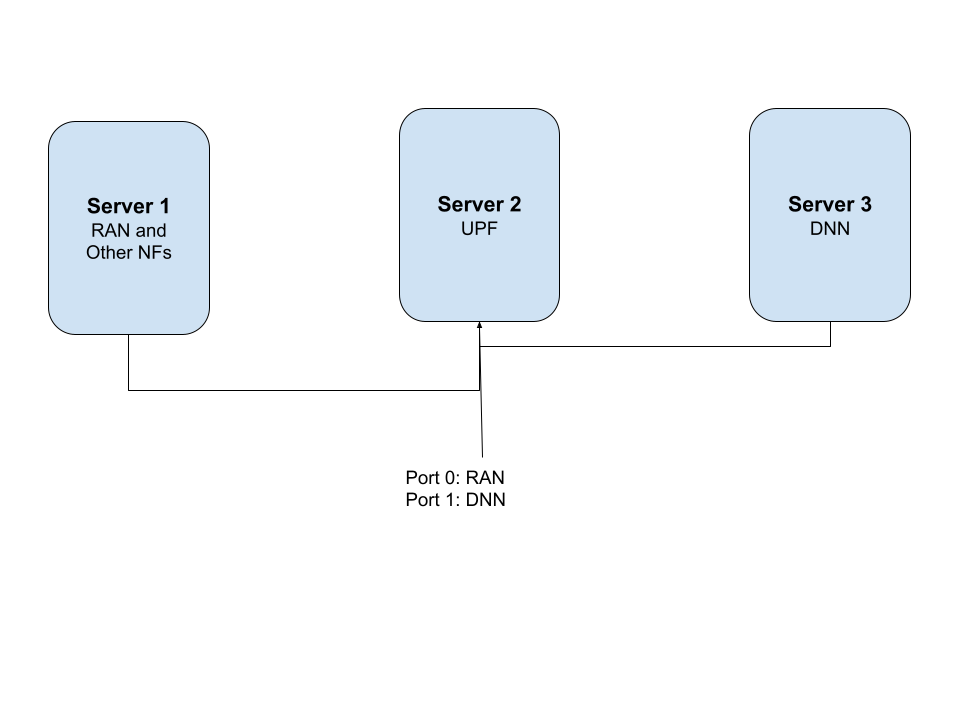
\includegraphics[width=0.7\textwidth, keepaspectratio]{./fig/Results/Setup.png}
    \caption{Experimental Setup}
    \label{fig:ExperimentalSetup}
\end{figure}
 The main features of the setup are: 
 \begin{itemize} 
        \item \textbf{Server's Layout}
        \begin{enumerate}
                \item \textbf{Server 1} The radio access network (RAN) and other network functions responsible for authentication,
         session establishment, charging functions are simulated on server 1.  The user equipments are also 
         simulated on the same machine. The load generation in the uplink direction is the main function of this server in the data forwarding plane.
                \item \textbf{Server 2} This server hosts the user plane function
		 (UPF). Two ports on this server are used to communicate with RAN 
         (server 1) and DNN (server 3).
                 \item \textbf{Server 3} This server simulates the data network name (DNN) network function. This network 
        function is the gateway to public Internet for 5G telecommunication. This server is used to generate downlink traffic. This server is also used to mirror packets received from uplink and forwarded back in the downlinj direction. The mirroring of latency packets help in measuring end-to-end latency (Round Trip Time) at the RAN. 
        \end{enumerate} 
        \item \textbf{Hardware Configuration} 
        \begin{enumerate}
                \item \textbf{CPU} Intel Xeon Core i5 @2.20GHz. 12 cores on every NUMA node. Only a single NUMA node is used in the experiments. Hyperthreading is kept off to facilitate repeatability of results.
                \item \textbf{Memory} 8192 superpages of size 2MB are reserved initially for the whole run.
                \item \textbf{Cache} 32 KB L1i-cache, 32 KB L1d-cache, 256 KB L2 cache per core. 30 MB L3 cache per NUMA node. 
                \item \textbf{NIC} Netronome Agilio CX 2x10GbE smartNIC.
	       \end{enumerate}
        
\end{itemize}

\section{UPF}
The primary role of user plane function is described in \ref{sec:UPF}. UPF is the main network function which takes the centre stage in the core network. The RAN load generator is used to test the processing capability of UPF. The metrics used are throughput and latency of data plane and control plane traffic. 

Different designs of the UPF are studied:

\begin{itemize}
	\item \textbf{Software UPF}

	This design uses kernel bypass framework DPDK for userspace processing of the incoming packets. All the control plane and data plane packets are received on the master core which redirects these packets into different worker cores.
	\item \textbf{Offloaded Data Plane}
	The complete data plane processing is offloaded on the smartNIC. The control plane messages are still processed in the software. Once a session is established (released), the rules are inserted (removed) in the smartNIC.
	
	\item \textbf{Offloaded Control Plane}
	In this design, the control plane handling is offloaded to the NIC. 
\end{itemize}
The detailed description of these designs are available in \cite{}.
\begin{table}[htbp]
\begin{scriptsize}
\begin{center}
\def\arraystretch{1.5}%  1 is the default, change whatever you need
\begin{tabular}{|p{3cm}|p{2cm}|p{2cm}|p{2cm}|}\hline 
% {\bf{Performance metric}} & {\bf{DPDK-based software UPF}} & {\bf{Dataplane offload}} & {\bf{Control plane offload}} \\ \hline 
{\bf{Performance metric}} & {\bf{SoftUPF}} & {\bf{DPOffload}} & {\bf{CPOffload}} \\ \hline 
{\bf{Throughput (messages/sec)}} & 5.1K  & 666  & 2.08M  \\ \hline
{\bf{Latency ($\mu s$)}} & 113  & 1646  & 24 \\ \hline
% {\bf{Performance per USD}} & 88  & 1 & 4.6K  \\ \hline
% {\bf{Performance per Watt}} & 40  & 1 & 41K \\ \hline
\end{tabular}
% \setlength{\abovecaptionskip}{-8pt}
% \setlength{\belowcaptionskip}{8pt}
\caption{Control plane performance.} 
% \vspace{-2mm}
\label{tab:perf-cp-offload}
\end{center}
\end{scriptsize}
\end{table}

\section{Results}
\subsection{Control Plane Performance}
The latency v/s. throughput graphs for different UPF designs  are illustrated in \ref{fig:SoftwareUPF},
\ref{fig:DPOFfload}, \ref{fig:CPOffload}. The summary of the results is shown in \ref{tab:perf-cp-offload}. The table \ref{tab:perf-cp-offload}
shows the latency around the control plane saturation. The control plane throughput is defined in terms
of sessions handled per second - the whole establishment, modification and response cycle for a given session 
is counted once.
\begin{figure}[htbp]
    \centering
    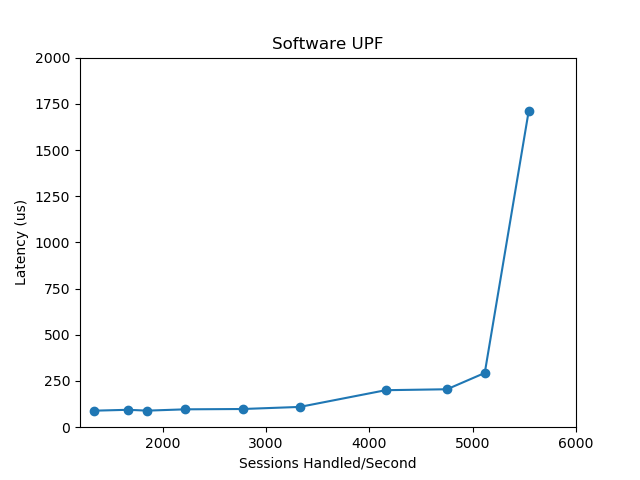
\includegraphics[width=0.7\textwidth, keepaspectratio]{./fig/Results/SoftUPF.png}
    \caption{Control Plane Performance for Software UPF}
    \label{fig:SoftwareUPF}
\end{figure}
\begin{figure}[htbp]
    \centering
    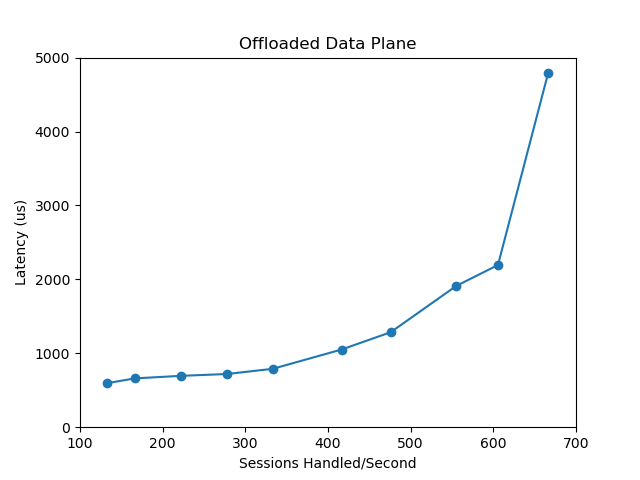
\includegraphics[width=0.7\textwidth, keepaspectratio]{./fig/Results/DPOffload.png}
    \caption{Control Plane Performance for Offloaded Data Plane}
    \label{fig:DPOFfload}
\end{figure}
\begin{figure}[htbp]
    \centering
    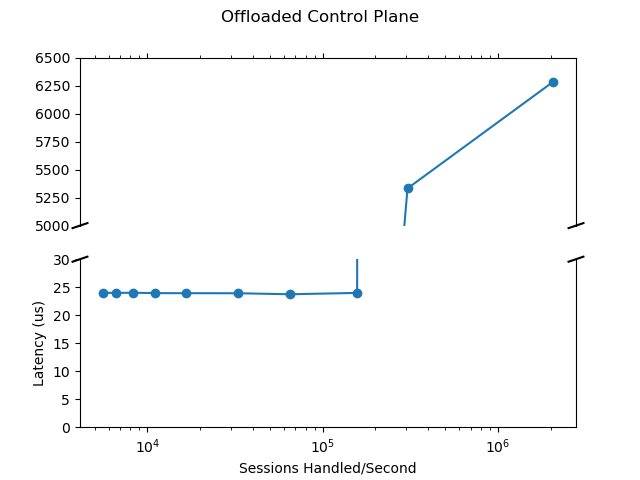
\includegraphics[width=0.7\textwidth, keepaspectratio]{./fig/Results/CPOffload.png}
    \caption{Control Plane Performance for Offloaded Control Plane}
    \label{fig:CPOffload}
\end{figure}

When the control plane is offloaded, we can see the best performance in terms of latency and throughput.
With the control plane offload, the latency is only around  24 us and 2.08 M sessions can 
be handled per second.
The performance deteriorates for data plane offload when compared to software UPF. This is 
attributed to the  bottleneck created between offloaded data plane
 and user space control plane - once the control plane messages are processed in
the user space, the rules are installed in smartNIC.

%
%\chapter{Conclusions\label{Con}}
%
%This report is concluded by describing three software techniques for fast packet processing besides DPDK.  
%\begin{figure}[htbp]
%    \centering
%    \includegraphics[width=0.7\textwidth, keepaspectratio]{./fig/c8f1.png}
%    \caption{Netslices \cite{marian2012netslices}}
%    \label{fig1c8} 
% \end{figure}
%\section{Netslices \label{netslices8}}
%
%
%The  packet capture libraries (\ref{softpmd3}) provide raw packets into the user space using raw sockets.
%However the path taken by packet can traverse across different cores. This is a performance bottleneck due to slow accesses to 
%non local memory in NUMA RAMs and cache misses in the local per core cache. This implies that raw sockets do not scale with the number of cores. 
%
%The key idea in Netslices\cite{marian2012netslices} is the spatial partitioning of physical resources  like CPU across different NIC queues. Figure \ref{fig1c8} shows how the resources are partitioned. A minimum of 2 cores are provided to a pair of Tx/Rx per NIC ring to match the line speeds. If the memory is NUMA-aware, local memory of the cores is implicitly reserved for handling packet.
%
%
%
% The problem of multiple memory copies - from NIC to kernel and from kernel to user space still remains.
% The solution scales with the number of cores on the system.
%
% \begin{figure}[htb]
%    \centering
%    \includegraphics[width=0.7\textwidth, keepaspectratio]{./fig/c8f2.png}
%    \caption{Vanilla PF\_RING \cite{pfringcite}}
%    \label{fig2c8} 
% \end{figure}
%\section{PF\_RING  and PF\_RING ZC\label{pfring8}}
%PF\_RING (figure \ref{fig2c8}) is a new socket which captures packets with the help of New API for polling in Linux. The packets are polled and copied in the kernel PF\_RING buffer. The user space application then retrieves these packets by another polling mechanism between kernel and user space. PF\_RING socket preallocates memory buffers for handling packets. This removes the allocation/deallocation overhead associated with \texttt{\emph{sk\_buff}} in Linux stack (refer \ref{skbuffhandling1}). However the problem of mmultiple meory copies still remains.
%
%PF\_RING ZC (Zero Copy) is an enhanced library which gives the userpace process direct access to NIC inteface. The packets are copied directly into memory buffers provided by the user space applications.
%This technique  can also scale linearly with the number of cores as the tuple (queue, application) can be independently handled (refer \cite{rizzo201210}).
%
%\begin{figure}[htbp]
%    \centering
%    \includegraphics[width=0.7\textwidth, keepaspectratio]{./fig/c8f3.png}
%    \caption{Netmap Rings \cite{rizzo2012netmap}}
%    \label{fig3c8} 
% \end{figure}
%\section{netmap \label{netmap8}}
%Netmap\cite{rizzo2012netmap} and DPDK try to solve the similar problems with Linux stack i.e. multiple memory copies, interrupt processing overhead and interrupt processing overheads and overhead associated with allocation and deallocation of buffers (section \ref{limitations1}). However, netmap solves this problem with the help of Linux kernel system calls - \emph{ioctl}, \emph{mmap}, \emph{epoll} and \emph{select} among others. But the packet processing occurs in user space.
%DPDK, as seen earlier, does not take any kernel support for packet processing except at the initialization. 
%
%\subsection{Working Principles  of \emph{netmap}}
%Netmap uses preallocated buffers. These buffers are in a shared memory region between kernel and user space. NIC rings (that stores the pointers to the data packets) are replicated in the form of netmap rings (Figure \ref{fig3c8}). These rings are used to communicate between the user space application and kernel. The actual NIC rings are protected from misbehaving applications by the kernel. This protection is the advantage of netmap over DPDK. In the case of DPDK PMDs, the NIC rings are directly mapped in user space. However different processes using the same netmap ring are not protected from each other. The solution to this problem is to use different netmap rings for different processes on different cores. This also enables parallelism in netmap.
%
%
%The netmap rings store relative offsets of packets from the base addresses enabling easy translation from kernel space to user space and vice versa. Hence netmap uses zero-copy technique.
%
%
%The packets of batches can be processed together by using polling system calls. This reduces interrupt processing overheads.
%
%
%\section{Closure \label{closure8}}
%
%\begin{table}[ht]
%   \resizebox{\textwidth}{!}{
%   \begin{tabular}{|c|c|c|c|} 
%    \hline
%       & Zero-Copy & Batching & Parallelism \\ 
%    \hline
%    Netslices & No & Yes by Polling & Yes \\ 
%    PF\_RING & Yes, ZC Library with direct NIC access enables zero copying. & Yes & Yes \\ 
%    \emph{netmap} & Yes & Yes (Polling) & Multiple netmap rings can be used. \\ 
%    DPDK & Yes& Yes & Yes \\ 
%     
%    \hline
%   \end{tabular}}
%   \caption{Comparison of Software Techniques}
%   \label{table18}
%   \end{table}
%   Packet processing in all the techniques discussed here operate in user-space. All the techniques discussed above can handle speeds upto 10 Gigabits/sec  wire speeds (refer \cite{cerovic2018fast}). 
%
%
%   DPDK is preferable over all the techniques and is widely used in industry for handling packet processing needs.
%   DPDK was started by Intel, which is the leader in manufacturing of network hardware and processors. Now it is a part of the Linux foundation with support from big players in telecom industry like AT \& T, ARM, and Ericcson among others \cite{membersdpdk}.
%   DPDK's success is attributed to the application of latest technological advances (discussed in \ref{optimizations2}). 
%   DPDK provides the support on application level by using state-of-the-art algorithms optimized for multi-core architectures (Chapter \ref{application}).
%

% %*******************************************************************************



% *******************************************************************************
\begin{spacing}{1}
\bibliographystyle{ieeetr}
\bibliography{conf}
\end{spacing}
\end{document}
%*******************************************************************************

